\documentclass[a4paper]{article}

\usepackage{amsmath}
\usepackage{float}
\usepackage{minted}
\usepackage{anyfontsize}
\usepackage{booktabs}
\usepackage{graphics}
\usepackage{siunitx}
\usepackage{caption}
\usepackage{enumitem}
\usepackage{textcomp}
\usepackage{pgfplots}
\usepackage{caption}
\usepackage[colorlinks,linkcolor=red]{hyperref}\usepackage{minted}

\pgfplotsset{compat=1.15}

\usepackage{ctex}
\usepackage{xeCJK}

\setCJKmainfont[ItalicFont={楷体}, BoldFont={黑体}]{宋体}

\newcommand{\tabincell}[2]{\begin{tabular}{@{}#1@{}}#2\end{tabular}}

\title{人工智能导论\\情感分析作业}
\author{计75罗崚骁\\2017011364}

\date{}

\begin{document}
    \maketitle
    % \begin{titlepage}
    % \end{titlepage}

    \section{模型结构图}

    \begin{figure}[H]
        \centering
        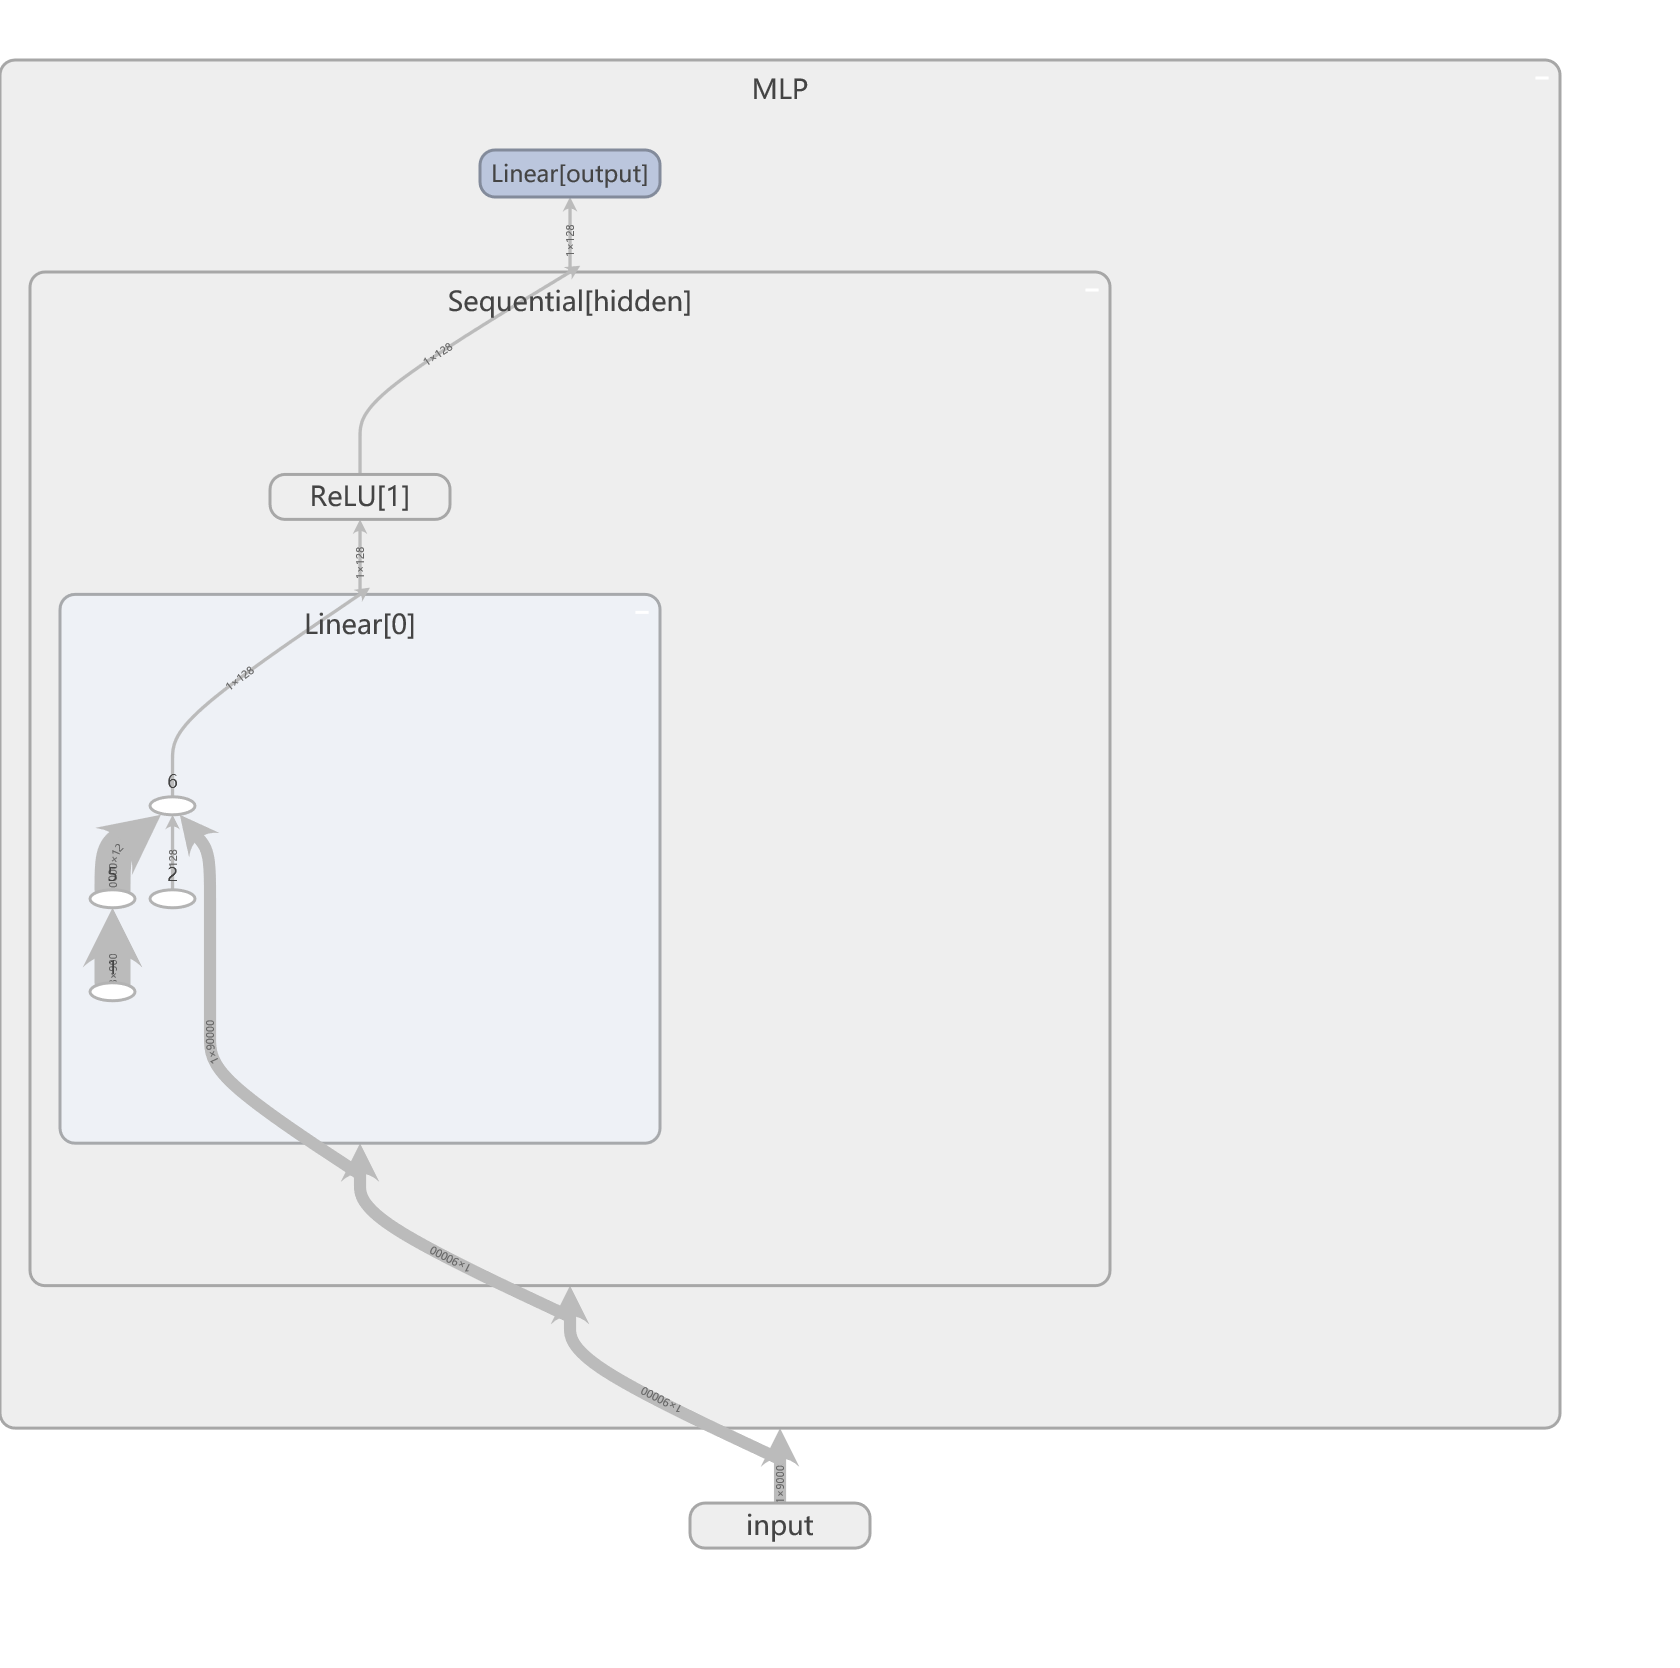
\includegraphics[width=\linewidth]{assets/mlp.png}
        \caption{MLP}
        % \label{}
    \end{figure}

    \begin{figure}[H]
        \centering
        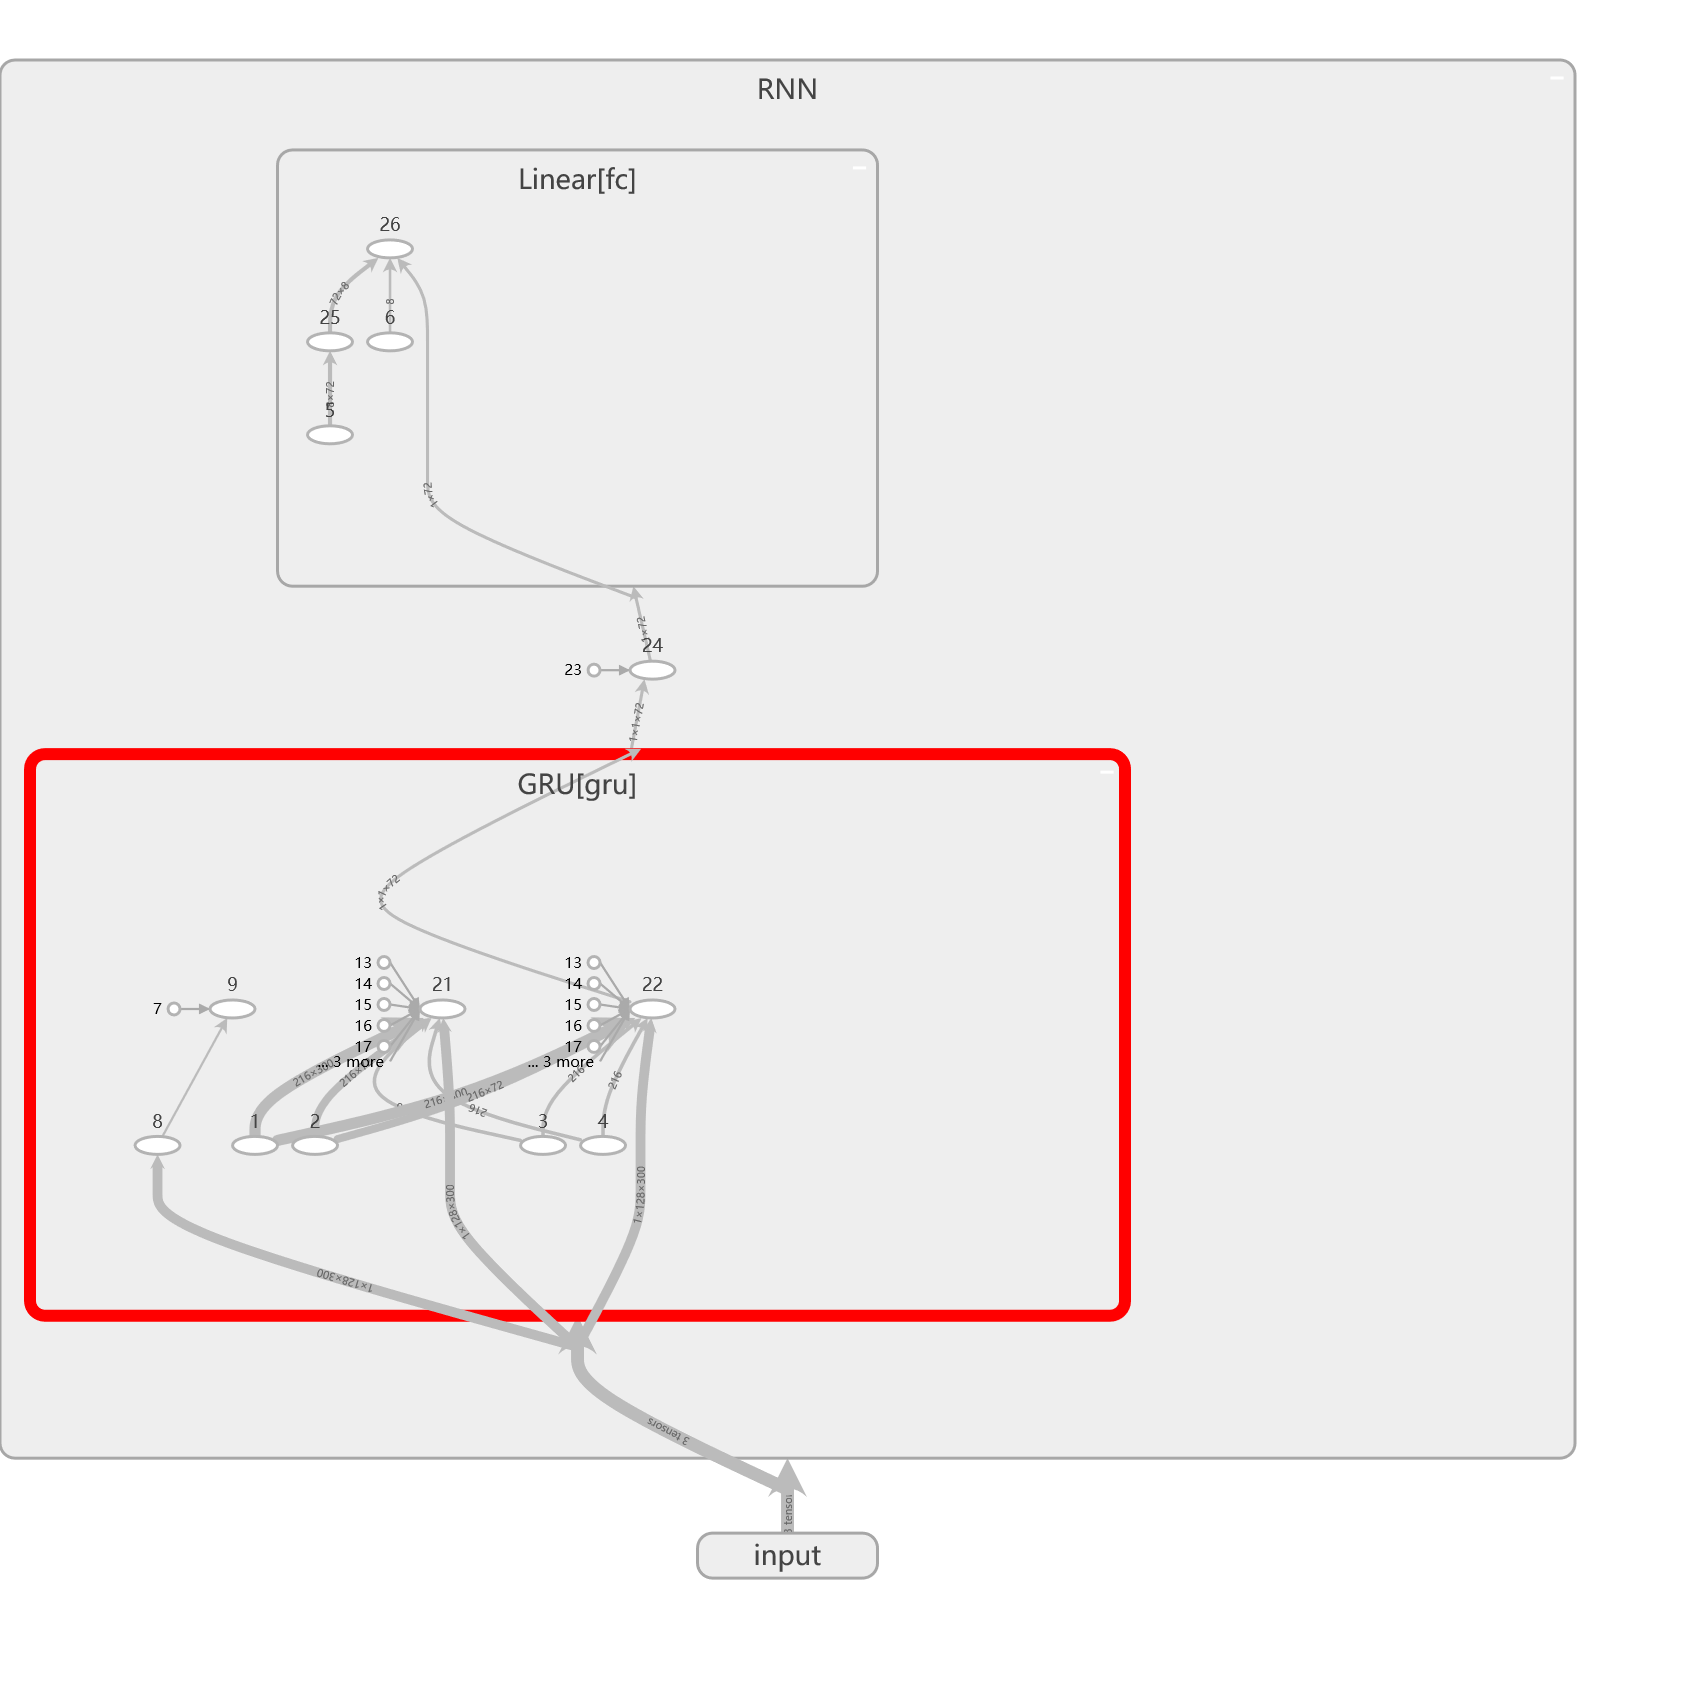
\includegraphics[width=\linewidth]{assets/rnn.png}
        \caption{RNN}
        % \label{}
    \end{figure}

    \begin{figure}[H]
        \centering
        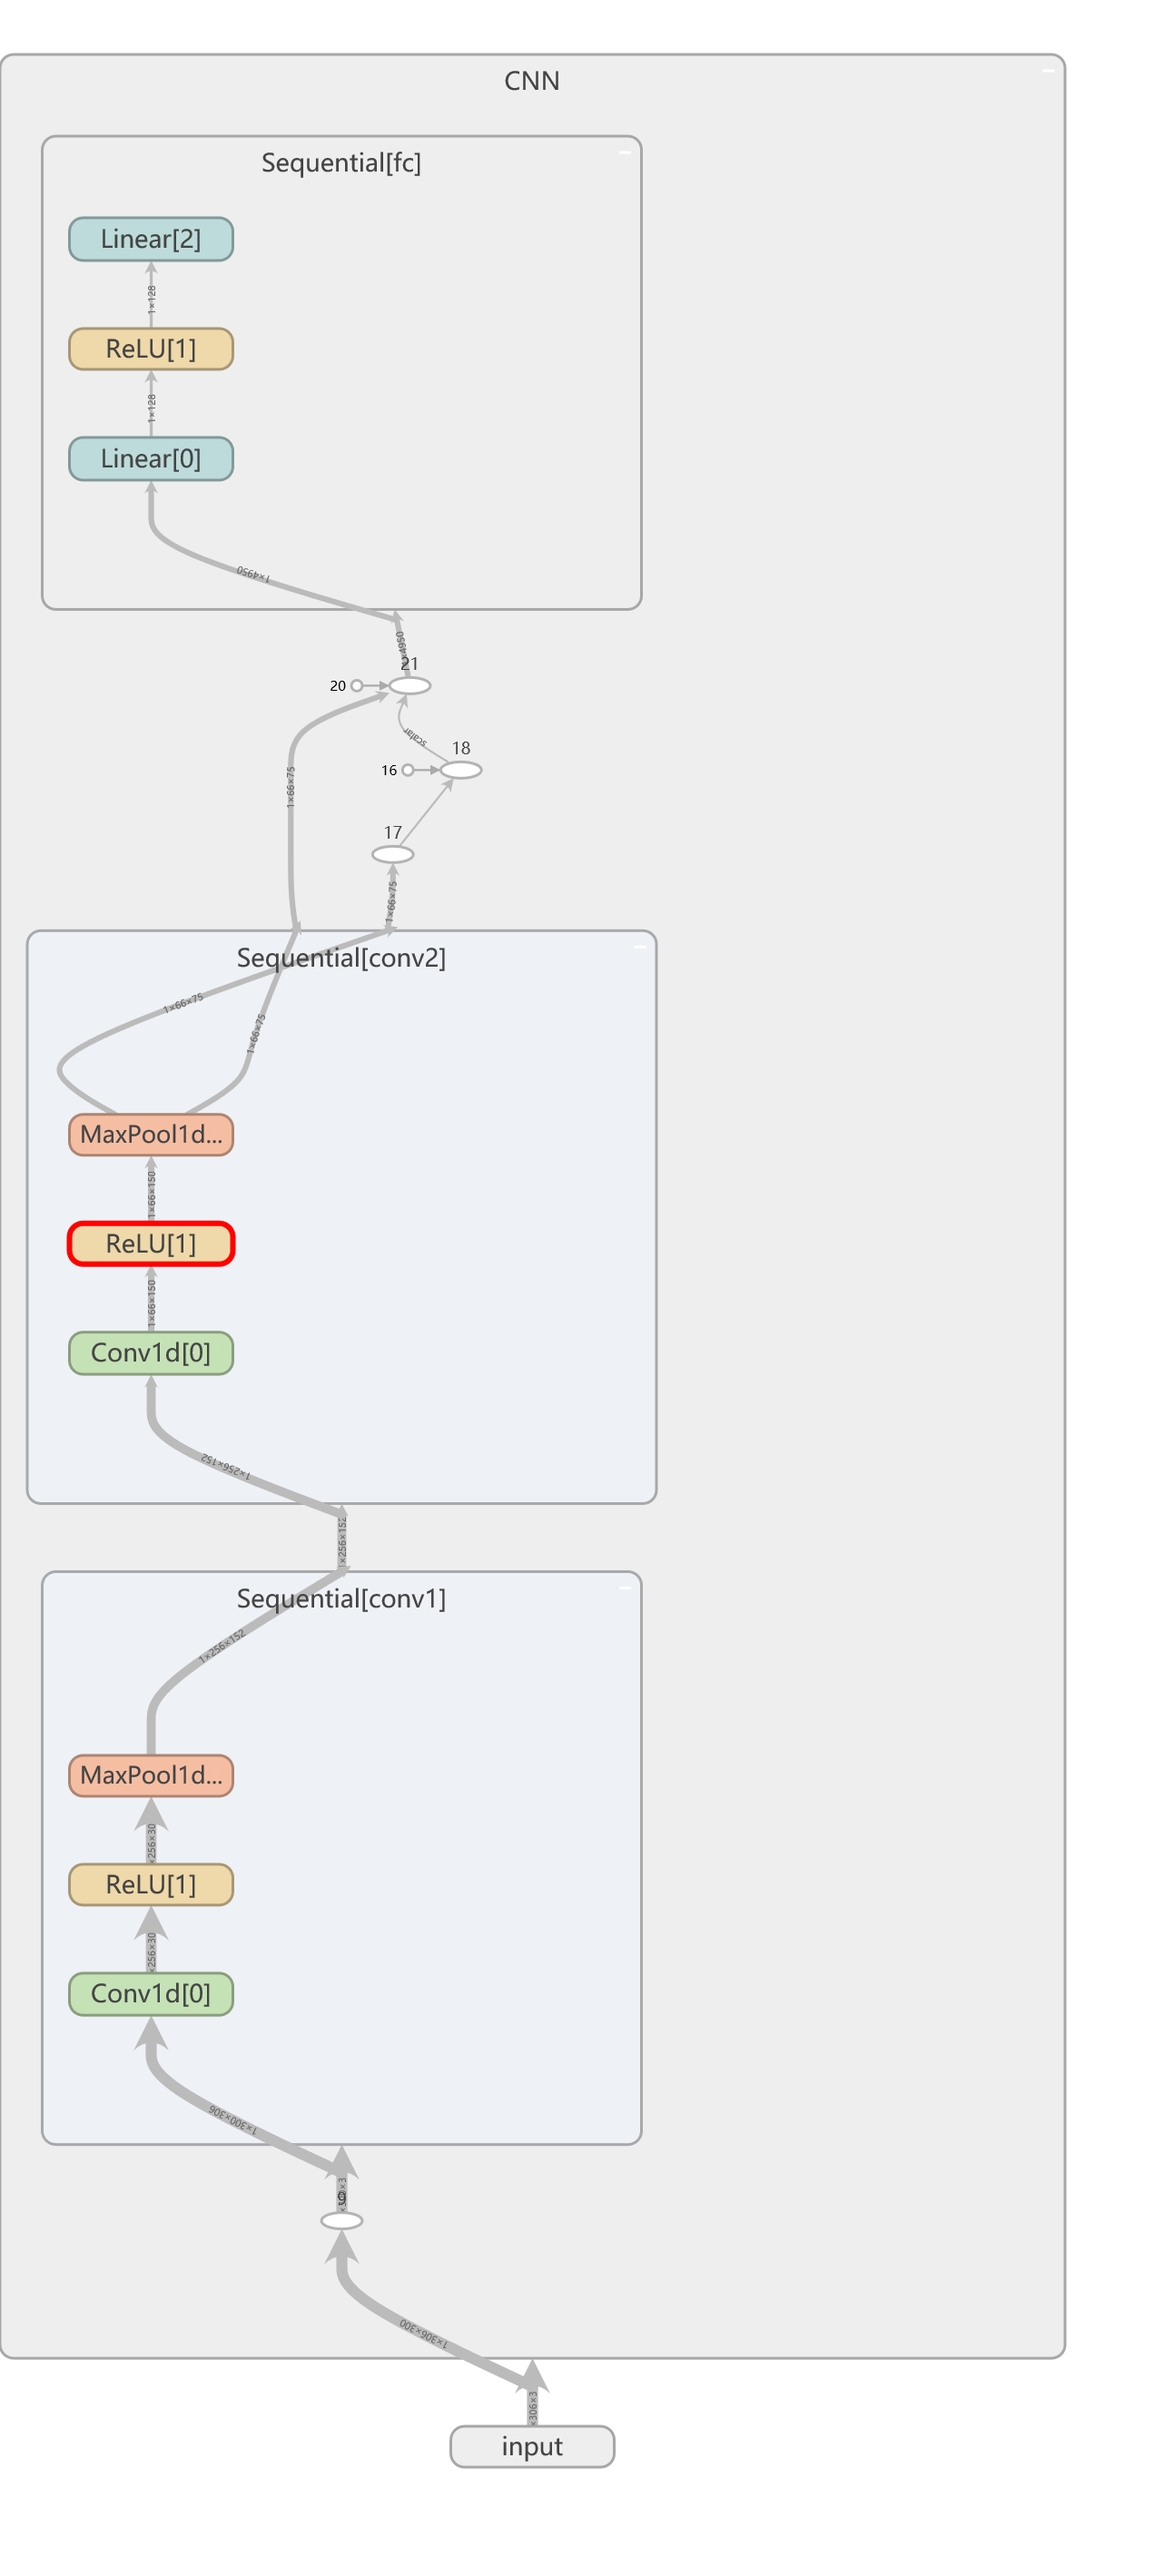
\includegraphics[width=.75\linewidth]{assets/cnn.png}
        \caption{CNN}
        % \label{}
    \end{figure}

    \newpage

    \section{流程分析}
    整个训练框架基于pytorch。使用了\url{https://github.com/Embedding/Chinese-Word-Vectors}提供的搜狗新闻的
    中文词汇预训练向量数据进行词嵌入(word embedding)。
    
    \subsection{预处理}
    由于词数较大,词向量长度也为不可忽略的300,
    为了节省空间以及加快训练时加载数据的速度,对已经经过分词的新闻数据再次进行了一次处理:
    首先统计出新闻中所有出现的词汇并编号,设共 $n$ 个词语,再保存一个长度为 $n$ 的
    词向量的列表,列表中第 $i$ 个元素为第$i$个词语对应的词向量。在程序运行时,只需先加载这个
    列表作为词典,对于训练数据中的每个词语,只需要加载其编号,用到时再去查询。
    这样可以节省很多内存,也并没有引入太多时间消耗,以至于虽然实验设备只是一台甚至没有N卡的普通的轻薄本,在整个实验过程中都未曾遇到
    内存问题。
    

    \subsection{数据准备}

    训练数据和测试数据的装载使用了torch.utils.data包中的Dataset与DataLoader两个类。

    将原始的训练数据分为两份,大小比例为 9:1,分别作为\textbf{训练}集与\textbf{验证}集,原始的测试机保持不变直接作为测试集。

    实例化三个Dataset类的对象将三个数据集装好,对于训练集,还要用从其Dataset类的对象
    实例化出新的DataLoader对象,用于训练。这是因为Dataset的作用是将数据全部装好,提供编号与迭代的支持,但是一般并不用于直接训练,可以用于作为
    测试时的迭代工具;DataLoader在训练时可以提供多批数据同时训练的支持(batch)。

    另外,由于文章长度各不相等,所以需要对文章进行截取,使得训练集中的文章长度都相等(虽然对于RNN并不需要,
    但是截取为统一长度方便处理,且也能取得较好效果,见后面分析)。一个截取的方法是:对于一个长度为
     $n$ 的文章,随机生成一个长度为 $n$ 的排列 $p$,截取 $p$ 的前若干位,保存截取后的排列对应的那些词语。
    注意到这个过程有随机性,为了保证神经网络的输出相同,需要让截取的方式相同,因此需要先固定随机种子。

    \subsection{网络搭建}
    使用了pytorch框架搭建神经网络,实现了MLP(baseline),RNN与CNN三种模型。
    实现的方式均为:
    \begin{enumerate}
        \item 继承torch.nn.Module类,实现构造函数与重写forward方法,
        \item 对模型使用Adam优化器,设置学习率,其余参数保持默认
        \item 持续对训练集整体进行多次迭代,每完成一次迭代用验证集进行验证,并保存最优模型;
        \item 达到某种判停准则要求后停止训练,并在测试集上测试结果。
    \end{enumerate}

    具体地,各个模型做了如下构建:
    \begin{itemize}
        \item MLP使用了一个隐层;
        \item RNN使用了GRU模型,输出层使用全连接;
        \item CNN使用了两个卷积层和两个全连接层。
    \end{itemize}
    
    激活函数使用了relu函数,几乎每层(除了输出层)都使用了激活函数,通过
    卷积层后还有一层池化层。
    
    模型的损失函数为交叉熵,对于同一批的训练数据计算出一个交叉熵,在此基础上进行反向传播。

    \newpage

    \section{实验结果}

    实验结果显示,三种模型都能成功训练并得到58\%左右的准确率。每种模型的训练时间
    不等,但大体都在可接受范围内(10分钟以内)。

    \begin{table}[H]
        \centering
        \begin{tabular}{cccc}
            \toprule
            模型名称 & 准确率(\%) & F-score & 相关系数\\
            \midrule
            MLP & 58.2 & 0.225 & 0.594 \\
            RNN & 58.0 & 0.246 & 0.620 \\
            CNN & 58.9 & 0.234 & 0.617 \\
            \bottomrule
        \end{tabular}
    \end{table}

    \begin{figure}[H]
        \centering
        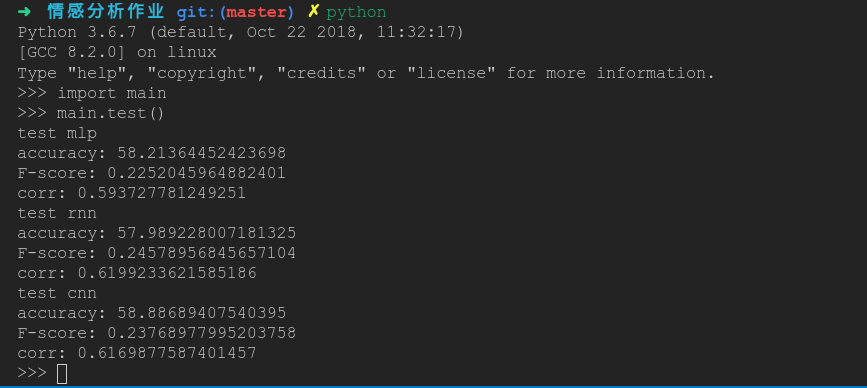
\includegraphics[width=\linewidth]{assets/test.png}
        % \caption{}
        % \label{}
    \end{figure}

    \newpage

    \section{参数比较}

    \subsection{学习率}
    学习率是一个比较微妙的参数,且对于不同模型选取也有所不同,主要影响因素
    为模型的收敛速度,学习率应与收敛速度呈负相关的关系。

    学习率如果较大,遇到过的问题有:
    \begin{itemize}
        \item 梯度爆炸(尤其对于RNN),经常得到NaN的结果;
        \item 太快达到过拟合,没能进行更多尝试而保存一些较优的中间结果(尤其对于MLP)
    \end{itemize}

    学习率较低遇到的问题有:
    \begin{itemize}
        \item 训练较慢,每次迭代学习到的东西较少,迟迟不达到收敛;
        \item 训练过于“谨慎”,容易掉进局部最优解。
    \end{itemize}

    最后学习率参数确定为
    \begin{table}[H]
        \centering

        \begin{tabular}{cccc}
            \toprule
            模型名称 & MLP & RNN & CNN\\
            \midrule
            学习率& $5\times 10^{-5}$ & $10^{-3}$ & $10^{-4}$\\
            \bottomrule
        \end{tabular}
    \end{table}

    从表中也能收敛速度为 MLP > CNN > RNN。

    \subsection{神经网络层数}

    虽然近年来深度学习在人工智能领域取得了巨大的成功,但是由于数据
    量与实验设备算力的限制,深层神经网络并不适合本次实验,最终的框架还是以浅层
    神经网络为主。
    \begin{itemize} 
        \item 对于MLP,只使用一个隐层已经可以达到较好效果;
        \item 对于RNN,二层比起一层效果略优,但训练速度明显变慢;
        \item 对于CNN,使用两个卷积层和两个全连接层也能达到较好效果。
    \end{itemize}

    % \subsection{迭代次数控制}

    % 为了防止过拟合,从训练集中取出了一部分作为验证集,以检测模型在
    % 非训练数据上的表现状况,并取在验证集上损失函数loss最低的(或准确率最高的)
    % 的模型保存为最终模型。如果连续对整个数据集迭代 $e$ 次都没能保存新的模型,
    % 则认为训练停止。

    % $e$ 的取值的矛盾在于:如果太小,则有时候因为模型暂时表现不好便认为结束训练,
    % 从而甚至以欠拟合结束;若太大则拖慢训练速度。经测试,取 $e=15$ 较为合适,此时
    % 一般都已经达到过拟合,且等待时间也可以接受。

    \subsection{文章截取词数}

    由于神经网络输入大小是固定的,数据处理时,一个要面对的问题是使输入的文章长度保持相同。
    虽然直观上来讲,截取的长度越长结果应该更准确,但是实际上并不总是这样。经过测试,文章截取长度
    边长时(例如对于RNN取到400),不仅训练速度严重变慢,结果还有所下降。
    
    最后结果是对于RNN取在 128 为宜,CNN与MLP可取 $300\sim400$。

    \subsection{神经网络超参数选取}

    神经网络中有很多固定的参数,例如RNN与MLP的隐层大小,CNN的中间通道,池化大小,卷积核大小,和全连接层大小。
    这些参数选取不同时,确实能出现不同的结果,且有较大差异。但由于知识的
    限制与神经网络本身(目前)固有的不可解释性,难以从中看出参数与结果的关系,
    实验中只是通过手动设置参数比较结果,选取最优。

    \section{RNN,CNN与baseline模型比较}
    由于本次实验具有的特殊性(问题较简单,训练数据和测试数据规模较小),因此
    MLP(baseline) 的表现效果很好,与RNN和CNN不分上下,甚至很多方面要更优秀。

    相比之下,baseline具有的特点是:收敛快,稳定性欠佳,以至于不得不选取较低的学习率,且参数少,实现简单;
    RNN与CNN的训练时间偏长,稳定性较好,调参较为困难。

    \newpage

    \section{问题思考}

    \subsection{迭代停止条件}

    为了防止过拟合,从训练集中取出了一部分作为验证集,以检测模型在
    非训练数据上的表现状况,并取在验证集上损失函数loss最低的(或准确率最高的)
    的模型保存为最终模型。如果连续对整个数据集迭代 $e$ 次都没能保存新的模型,
    则认为训练停止。

    $e$ 的取值的矛盾在于:如果太小,则有时候因为模型暂时表现不好便认为结束训练,
    从而甚至以欠拟合结束;若太大则拖慢训练速度。经测试,取 $e=15$ 较为合适,此时
    一般都已经达到过拟合,且等待时间也可以接受。

    对于固定迭代次数和使用验证集的两种方式,我认为使用验证集的方式更好。若固定迭代次数,
    则这个适合的迭代次数会随着模型的不同,参数选取的不同而变化,增加调参难度,且难以控制;
    使用验证集的方法则可根据模型在验证集上的表现非常准确地判断是否达到过拟合。

    \subsection{参数初始化}

    参数初始化的方法为,对于所有权重矩阵(weight),使用高斯分布初始化;对于所有偏置向量,
    使用零初始化。初始化的实现如下:

    \begin{minted}{py}

def weight_init(m):
    from torch import nn

    try:
        nn.init.xavier_uniform_(m.weight)
    except AttributeError:
        pass

    try:
        nn.init.constant_(m.bias, 0)
    except AttributeError:
        pass

net.apply(weight_init)  # net 为某种模型
    \end{minted}

    通常而言,权重矩阵适合使用高斯分布初始化。值得一提的是,对于正交初始化,由于
    正交变换是保长度的,因此比较适用于RNN这种容易出现梯度爆炸的模型。

    
    \subsection{过拟合预防方法}

    \begin{itemize}
        \item 首先有停止迭代条件的两种选择:设置迭代次数,使用验证集。使用验证集时,应该以验证集的表现为准,通常验证集的准确率随着拟合程度的增加呈现单峰的趋势;
        \item 在损失函数中添加正则项,例如对于对于误差函数 $E(\vec{w})$可添加正则项 $\lVert \vec{w} \rVert$,修改为 $E'(\vec{w})=E(\vec{w})+\lVert \vec{w} \rVert$,
        其中范数可以为向量的1-范数或2-范数,或其它范数;
        \item 舍弃(Dropout)机制:在训练的过程中,随机地舍弃一些隐层单元。
    \end{itemize}

    \subsection{三种模型的优缺点}

    \begin{itemize}
        \item MLP(单层)的优点为调参简单,训练快,适用于这种数据量小,简单的实验,对于新手来讲容易理解与上手;缺点是计算量偏大,不容易扩展至大数据,且对于小数据学习率只能调低以防止过快拟合,也没能利用到上下文信息。
        \item RNN的优点是具有记忆性,可以支持任意长度的文本输入,理论上最适合处理文本和语音数据;缺点是训练
        缺点是计算速度较慢,训练时间长,训练过程中由于可以支持任意长度的输入,容易出现梯度爆炸现象;此外,最后一个词的作用
        往往显得比较重要。
        \item CNN 的优点是,使用卷积核处理输入数据,可以很方便地处理高维输入,比较适合做图像和视频处理,在本实验中最后的效果
        也是最好的;缺点是理论上并不适合作文本处理,且需要对文本作预处理(统一长度),超参数的选取也多依赖于经验。
    \end{itemize}

    
    \section{心得体会}

    \begin{itemize}
        \item 神经网络是强大的工具,但是参数调整过程中存在很多不可解释的地方,还需要学习和研究;
        \item 对于不同问题(例如本次实验,和其它的图像视频处理问题等),不同模型,不同参数有不同的表现效果,要大胆尝试,小心甄别;
        \item baseline不一定是最弱的,深度神经网络不一定比浅层神经网络要好。就好比如今的人工智能(尤其国内)多数在强调深度学习,
        但事实上深度学习几乎已达瓶颈,且还有很多其它算法有待研究,不可随波逐流,先入为主地认为深度学习和神经网络就是最好的。
    \end{itemize}
    
    
\end{document}